\begin{figure}[t]
\centering
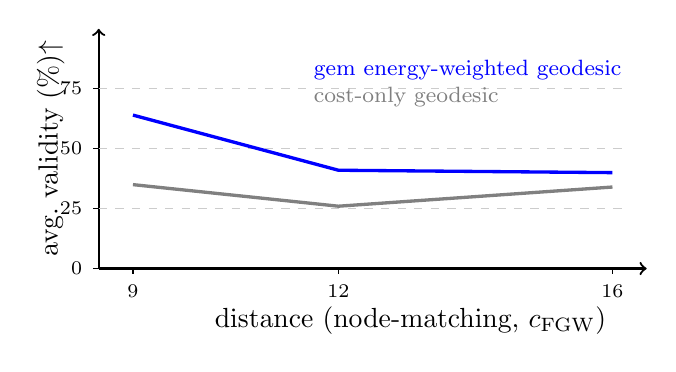
\begin{tikzpicture}[scale=0.87]
  % Axes
  \draw[->, thick] (8.5,0) -- (16.5,0) node[below, xshift=-3cm, yshift=-0.35cm] {distance (node-matching, $c_{\mathrm{FGW}}$)};
  \draw[->, thick] (8.5,0) -- (8.5,3.5);
  \node[rotate=90] at (7.8,1.75) {avg.\ validity (\%)$\uparrow$};

  % Y-axis ticks and labels
  \foreach \y/\label in {0/0, 0.875/25, 1.75/50, 2.625/75} {
    \draw (8.5,\y) -- (8.42,\y);
    \node[left,font=\scriptsize] at (8.4,\y) {\label};
    
    % FIX: Only draw the dashed grid line if y > 0
    \ifdim \y pt > 0pt
        \draw[gray!40, dashed] (8.5,\y) -- (16.2,\y);
    \fi
  }

  % X-axis ticks and labels
  \foreach \x in {9,12,16} {
    \draw (\x,0) -- (\x,-0.08);
    \node[below,font=\scriptsize] at (\x,-0.1) {\x};
  }

  % Data coordinates (scaled by Y: 3.5 units = 100%)
  \draw[very thick, blue] plot coordinates {(9,2.24) (12,1.435) (16,1.4)};
  \draw[very thick, gray] plot coordinates {(9,1.225) (12,0.91) (16,1.19)};

  % Legends
  \node[blue, anchor=west, font=\footnotesize] at (11.5,2.9) {\gls{gem} energy-weighted geodesic};
  \node[gray, anchor=west, font=\footnotesize] at (11.5,2.5) {cost-only geodesic};
\end{tikzpicture}
\caption{\footnotesize \textbf{Validity Along Geodesics.} Average chemical validity (\%) vs.\ distance (node-matching, $c_{\mathrm{FGW}}$) for \gls{gem} energy-weighted versus cost-only geodesics. Cost-only ignores the learned data geometry and interpolates through low-validity regions.}
\label{fig:geodesic-validity}
\end{figure}